\setcounter{chapter}{15}

\chapter{Frequency-Severity Models}

{\small \textit{Chapter Preview}. Many data sets feature dependent
variables that have a large proportion of zeros. This chapter
introduces a standard econometric tool, known as a \emph{tobit
model}, for handling such data. The tobit model is based on
observing a left-censored dependent variable, such as sales of a
product or claim on a healthcare policy, where it is known that the
dependent variable cannot be below zero. Although this standard tool
can be useful, many actuarial data sets that feature a large
proportion of zeros are better modeled in ``two parts,'' one part
for the frequency and one part for the severity. This chapter
introduces two-part models and provides extensions to an
\emph{aggregate loss model}, where a unit under study, such as an
insurance policy, can result in more than one claim.}


\section{Introduction}\index{regression model!two-part}\index{regression model!frequency-severity}

Many actuarial data sets come in ``two parts:''

\begin{itemize}
\item one part for the frequency, indicating whether or not a claim has
occurred or, more generally, the number of claims and

\item one part for the severity, indicating the amount of a claim.
\end{itemize}

\marginparjed{Two-part models consist of frequency (number) and
severity (amount) components.}

In predicting or estimating claims distributions, we often associate
the cost of claims with two components: the event of the claim and
its amount, if the claim occurs. Actuaries term these the claims
\emph{frequency} and \emph{severity components}, respectively. This
is the traditional way of decomposing ``two-part'' data, where one
can think of a zero as arising from a policy without a claim (Bowers
et al., 1997, Chapter 2). Because of this decomposition, two-part
models are also known as \emph{frequency-severity models}. However,
this formulation has been traditionally used without covariates to
explain either the frequency or severity components. In the
econometrics literature, Cragg (1971) introduced covariates into
these two components, citing an example from fire insurance.

Healthcare data also often feature a large proportion of zeros that must be
accounted for in the modeling. Zero values can represent an individual's
lack of healthcare utilization, no expenditure or non-participation in a
program. In healthcare, Mullahy (1998) cites some prominent areas of
potential applicability:

\begin{itemize}\index{actuarial \& financial terms and concepts!demand}
\item outcomes research - amount of health care utilization or expenditures

\item demand for health care - amount of health care sought, such as number
of physician visits and

\item substance abuse - amount consumed of tobacco, alcohol and illicit
drugs.
\end{itemize}

The two-part aspect can be obscured by a natural way of recording
data; enter the amount of the claim when the claim occurs (a
positive number) and a zero for no claim. It is easy to overlook a
large proportion of zeros, particularly when the analyst is also
concerned with many covariates that may help explain a dependent
variable. As we will see in this chapter, ignoring the two-part
nature can lead to serious bias. To illustrate, recall from Chapter
6 a plot of individual's income ($x$) versus amount of insurance
purchased ($y$) (Figure 6.3). Fitting a single line to these data
would misinform users about the effects of $x$ on $y$.

\begin{figure}[htp]
    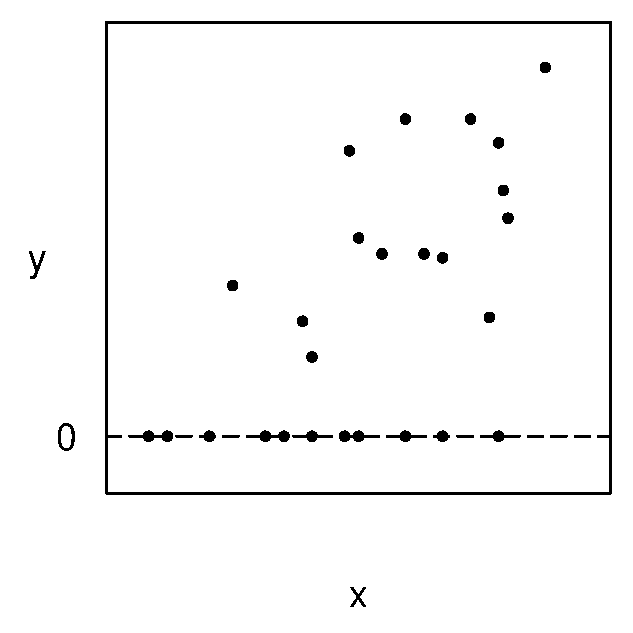
\includegraphics[width=0.45\textwidth]{Chapter6/F6TwoPartZero.eps}
        \caption{\label{F6:TwoPartZero} When individuals do not purchase insurance, they are recorded as $y=0$ sales.
        The sample in this plot represents two subsamples, those who
purchased insurance, corresponding to $y>0$, and those who did not,
corresponding to $y=0$. }
\end{figure}

In contrast, many insurers keep separate data files for frequency
and severity. For example, insurers maintain a ``policyholder'' file
that is established when a policy is underwritten. This file records
much underwriting information about the insured(s), such as age,
gender and prior claims experience, policy information such as
coverage, deductibles and limitations, as well as the insurance
claims event. A separate file, often known as the ``claims'' file,
records details of the claim against the insurer, including the
amount. (There may also be a ``payments'' file that records the
timing of the payments although we shall not deal with that here.)
This recording process makes it natural for insurers to model the
frequency and severity as separate processes.

\section{Tobit Model}\index{regression model!tobit}\index{censoring}

One way of modeling a large proportion of zeros is to assume that
the dependent variable is (left) censored at zero. This chapter
introduces left-censored regression, beginning with the well-known
\emph{tobit model} that is based on the pioneering work of James
Tobin (1958). Subsequently, Goldberger (1964) coined the phrase
``tobit model,'' acknowledging the work of Tobin and its similarity
to the probit model.

\marginparjed{A latent variable is not observed by the analyst.}

As with probit (and other binary response) models, we use an
unobserved, or latent, variable $y^{\ast}$ that is assumed to follow
a linear regression
model of the form%
\begin{equation}\label{E16:Eq1}
y_i^{\ast} = \mathbf{x}_i^{\prime} \boldsymbol \beta +
\varepsilon_i.
\end{equation}
The responses are censored or ``limited'' in the sense that we
observe $y_i = \max \left( y_i^{\ast},d_i\right)$. The limiting
value, $d_i$, is a known amount. Many applications use $d_i=0$,
corresponding to zero sales or expenses, depending on the
application. However, we also might use $d_i$ for the daily expenses
claimed for travel reimbursement and allow the reimbursement (such
as \$50 or \$100) to vary by employee $i$. Some readers may wish to
review Section 14.2 for an introduction to censoring.

The model parameters consist of the regression coefficients,
$\boldsymbol \beta $, and the variability term, $\sigma
^{2}=\mathrm{Var}~\varepsilon _i$. With equation (\ref{E16:Eq1}), we
interpret the regression coefficients as the marginal change of
$\mathrm{E~}y^{\ast}$\ per unit change in each explanatory variable.
This may be satisfactory in some applications, such as when
$y^{\ast}$\ \ represents an insurance loss. However, for most
applications, users are typically interested in marginal changes in
$\mathrm{E~}y$, that is, the expected value of the \emph{observed}
response.

To interpret these marginal changes, it is customary to adopt the
assumption of normality for the latent variable $y_i^{\ast}$\ (or
equivalently for the disturbance $\varepsilon_i$). With this
assumption, standard calculations (see Exercise 16.1) show that
\begin{equation}\label{E16:Eq2}
\mathrm{E~}y_i = d_i+\Phi \left( \frac{\mathbf{x}_i^{\prime}
\boldsymbol \beta - d_i}{\sigma }\right) \left(
\mathbf{x}_i^{\prime}\boldsymbol \beta -d_i\mathbf{+}\sigma
\lambda_i\right) ,
\end{equation}
where
\begin{equation*}
\lambda_i=\frac{\mathrm{\phi }\left( (\mathbf{x}_i^{\prime}
\boldsymbol \beta - d_i\mathbf{)/}\sigma \right) }{\Phi \left(
(\mathbf{x}_i^{\prime} \boldsymbol \beta - d_i \mathbf{)/}\sigma
\right) }.
\end{equation*}\index{inverse Mills ratio}
Here, $\mathrm{\phi (.)}$ and $\Phi (.)$\ are the standard normal
density and distribution functions, respectively. The ratio of a
probability density function to a cumulative distribution function
is sometimes called an \emph{inverse Mills ratio}. Although complex
in appearance, equation (\ref{E16:Eq2}) allows one to readily
compute $\mathrm{E~} y $. For large values of
$(\mathbf{x}_i^{\prime}\boldsymbol \beta - d_i\mathbf{)/}\sigma $,
we see that $\lambda_i$\ is close to $0$ and $ \Phi \left(
(\mathbf{x}_i^{\prime}\boldsymbol \beta -d_i\mathbf{)/ }\sigma
\right) $\ is close to $1$. We interpret this to mean, for large
values of the systematic component $\mathbf{x}_i^{\prime}\boldsymbol
\beta,$ that the regression function $\mathrm{E~}y_i$\ tends to be
linear and the usual interpretations apply. The tobit model
specification has the greatest impact on observations close to the
limiting value $d_i$.

\marginparjed{The tobit model specification has the greatest impact
on observations close to the limiting value $d_i$.}

Equation (\ref{E16:Eq2}) shows that if an analyst ignores the
effects of censoring, then the regression function can be quite
different than the typical linear regression function,
$\mathrm{E~}y=\mathbf{x}^{\prime}\boldsymbol \beta ,$\ resulting in
biased estimates of coefficients. The other tempting path is to
exclude limited observations ($y_i=d_i$) from the dataset and again
run ordinary regression. However, standard calculations also show
that

\begin{equation}
\mathrm{E~}\left( y_i|\ y_i>d_i\right)
=\mathbf{x}_i^{\prime}\boldsymbol \beta + \sigma \frac{\mathrm{\phi
}\left( (\mathbf{x}_i^{\prime} \boldsymbol \beta -
d_i\mathbf{)/}\sigma \right) }{1-\Phi \left( (\mathbf{x}_i^{\prime}
\boldsymbol \beta - d_i \mathbf{)/}\sigma \right) }
\end{equation}
Thus, this procedure also results in biased regression coefficients.

A commonly used method of estimating the tobit model is maximum
likelihood. Employing the normality assumption, standard
calculations show that the log-likelihood can be expressed as
\begin{equation}\label{E16:Eq4}
\ln L = \sum\limits_{i:y_i=d_i} \ln \left\{ 1-\Phi \left(
\frac{\mathbf{x} _i^{\prime}\boldsymbol \beta -d_i}{\sigma }\right)
\right\} -\frac{1}{2} \sum\limits_{i:y_i>d_i} \left\{ \ln 2\pi
\sigma ^2 + \frac{(y_i-( \mathbf{x}_i^{\prime}\boldsymbol
\beta-d_i\mathbf{))}^2 }{\sigma^2}\right\} ,
\end{equation}
where $\{i:y_i=d_i\}$ and $\{i:y_i>d_i\}$\ means the sum over the
censored and noncensored observations, respectively. Many
statistical software packages can readily compute the maximum
likelihood estimators, $\mathbf{b}_{MLE}$ and $s_{MLE}$, as well as
corresponding standard errors. Section 11.9 introduces likelihood
inference. \index{likelihood inference!censoring}

For some users, it is convenient to have an algorithm that does not
rely on specialized software. A two-stage algorithm due to Heckman
(1976) fulfills this need. For this algorithm, first subtract $d_i$
from each $y_i$, so that one may take $d_i$ to be zero without loss
of generality. Even for those who wish to use the more efficient
maximum likelihood estimators, Heckman's algorithm can be useful in
the model exploration stage as one uses linear regression to help
select the appropriate form of the regression equation.

\bigskip

\boxedjed

\textit{Heckman's Algorithm for Estimating Tobit Model Parameters}

\begin{enumerate}
\item For the first stage, define the binary variable
\begin{equation*}
r_i=\left\{
\begin{array}{ll}
1 & \mathrm{if}~y_i>0 \\
0 & \mathrm{if}~y_i=0
\end{array}
\right. ,
\end{equation*}
indicating whether or not the observation is censored. Run a probit
regression using $r_i$ as the dependent variable and $\mathbf{x}_i$
as explanatory variables. Call the resulting regression coefficients
$\mathbf{g}_{PROBIT}.$

\item For each uncensored observation, compute the estimated variable
\begin{equation*}
\widehat{\lambda}_i=\frac{\mathrm{\phi }\left( \mathbf{x}_i^{\prime}
\mathbf{g}_{PROBIT}\right) }{\Phi \left( \mathbf{x}_i^{\prime}
\mathbf{g}_{PROBIT}\right) },
\end{equation*}
an inverse Mill's ratio. With this, run a regression of $y_i$ on
$\mathbf{x}_i$\ and $\widehat{\lambda}_i$. Call the resulting
regression coefficients $\mathbf{b}_{2SLS}.$
\end{enumerate}

\end{boxedminipage}

\bigskip

The idea behind this algorithm is that equation (\ref{E16:Eq1}) has
the same form as the probit model; thus, consistent estimates of the
regression coefficients (up to scale) can be computed. The
regression coefficients $\mathbf{b}_{2SLS}$ provide consistent and
asymptotically normal estimates of $\boldsymbol \beta$. They are,
however, inefficient compared to the maximum likelihood estimators,
$\mathbf{b}_{MLE}$. Standard calculations (see Exercise 16.1) show
that $\mathrm{Var~}\left( y_i|\ y_i>d_i\right) $ depends on $i$
(even when $d_i$ is constant). Thus, it is customary to use
heteroscedasticity-consistent standard errors for
$\mathbf{b}_{2SLS}$.\index{heteroscedasticity-consistent standard
error}

\section{Application: Medical Expenditures}\ecaptionjed{MEPS Health Expenditures}

This section considers data from the Medical Expenditure Panel
Survey (MEPS) that were introduced in Section 11.4. Recall that MEPS
is a probability survey that provides nationally representative
estimates of health care use, expenditures, sources of payment, and
insurance coverage for the U.S. civilian population. We consider
MEPS data from the first panel of 2003 and take a random sample of
$n=2,000$ individuals between ages 18 and 65. Section 11.4 analyzed
the frequency component, trying to understand the determinants that
influenced whether or not people were hospitalized. Section 13.4
analyzed the severity component; given that a person was
hospitalized, what are the determinants of medical expenditures?
This chapter seeks to unify these two components into a single model
of healthcare utilization.


\subsubsection*{Summary Statistics}\empexjed{HealthExpend}\index{datasets!MEPS health expenditures}

Table 16.1 reviews these explanatory variables and provides summary
statistics that suggest their effects on expenditures of inpatient
visits. The second column, ``Average Expend,'' displays the average
logarithmic expenditure by explanatory variable, treating no
expenditures as a zero (logarithmic) expenditure. This would be the
primary variable of interest if one did not decompose the total
expenditure into a discrete zero and continuous amount.

Examining this overall average (logarithmic) expenditure, we see
that females had higher expenditures than males. In terms of
ethnicity, native Americans and Asians had the lowest average
expenditures. However, these two ethnic groups accounted for only
5.4\% of the total sample size. Regarding regions, it appears that
individuals from the West had the lowest average expenditures. In
terms of education, more educated persons had lower expenditures.
This observation supports the theory that more educated persons take
more active roles in keeping their health. When it comes to
self-rated health status, poorer physical, mental health and
activity related limitations led to greater expenditures. Lower
income individuals had greater expenditures and those with insurance
coverage had greater average expenditures.



Table 16.1 also describes the effects of explanatory variables on
the frequency of utilization and average expenditures for those that
used inpatient services. As in Table 11.4, the column ``Percent
Positive Expend'' gives the percentage of individuals that had some
positive expenditure, by explanatory variable. The column ``Average
of Pos Expend'' gives the average (logarithmic) expenditure in case
where there was an expenditure, ignoring the zeros. This is
comparable to the median expenditure in Table 13.5 (given in
dollars, not log dollars).

\marginparjed{A variable's effect on overall expenditures may be
positive, negative or non-significant; this effect can be quite
different when we decompose expenditures into frequency and amount
components.}

To illustrate, consider that females had a higher average
expenditures than males by looking at the ``Average Expend'' column.
Breaking this down into frequency and amount of utilization, we see
that females had a higher frequency of utilization but, when they
had a positive utilization, the average (logarithmic) expenditure
was \emph{lower} than males. An examination of Table 16.1 shows this
observation holds true for other explanatory variables. A variable's
effect on overall expenditures may be positive, negative or
non-significant; this effect can be quite different when we
decompose expenditures into frequency and amount components.


Table \ref{T16:MEPSRegr} compares the ordinary least squares (OLS)
regression to maximum likelihood estimates for the tobit model. From
this table, we can see that there is a substantial agreement among
the $t$-ratios for these fitted models. This agreement comes from
examining the sign (positive or negative) and the magnitude (such as
exceeding two for statistical significance) of each variable's
$t$-ratio. The regression coefficients also largely agree in sign.
However, it is not surprising that the magnitudes of the regression
coefficients differ substantially. This is because, from equation
(\ref{E16:Eq2}), we can see that the tobit coefficients measure the
marginal change of the expected latent variable $y^{\ast}$, not the
marginal change of the expected observed variable $y$, as does OLS.

\clearpage

\begin{sidewaystable}
\scalefont{0.8}\begin{center}
\begin{tabular}{lllrrrr}
\multicolumn{7}{c}{Table 16.1. \textit{Percent of Positive
Expenditures
and Average Logarithmic Expenditure, by Explanatory Variable}} \\
\hline
Category & Variable & Description & Percent & Average & Percent & Average \\
&  &  & of data & \multicolumn{1}{r}{Expend} & \multicolumn{1}{r}{Positive}
& of Pos \\
&  &  &  & \multicolumn{1}{r}{} & \multicolumn{1}{r}{Expend} & Expend \\
\hline Demography &        AGE &  \multicolumn{2}{l}{Age in years
between
18  to 65 (mean: 39.0)}          \\
           &     GENDER & 1 if female &       52.7 &       0.91 &       10.7 &       8.53 \\
           &     GENDER &  1 if male &       47.3 &       0.40 &       4.7 &       8.66 \\
 Ethnicity &      ASIAN & 1 if Asian &        4.3 &       0.37 &        4.7 &       7.98 \\
           &      BLACK & 1 if Black &       14.8 &       0.90 &       10.5 &       8.60 \\
           &     NATIVE & 1 if Native &        1.1 &       1.06 &       13.6 &       7.79 \\
           &      WHITE & Reference level &       79.9 &       0.64 &        7.5 &       8.59 \\
    Region &  NORTHEAST & 1 if Northeast &       14.3 &       0.83 &       10.1 &       8.17 \\
           &    MIDWEST & 1 if Midwest &       19.7 &       0.76 &        8.7 &       8.79 \\
           &      SOUTH & 1 if South &       38.2 &       0.72 &        8.4 &       8.65 \\
           &       WEST & Reference level &       27.9 &       0.46 &        5.4 &       8.51 \\
           \hline
 Education &    COLLEGE & 1 if college or higher degree &       27.2 &       0.58 &        6.8 &       8.50 \\
           & HIGHSCHOOL & 1 if high school degree &       43.3 &       0.67 &        7.9 &       8.54 \\
           &      \multicolumn{2}{l}{Reference level is lower than high school degree} &       29.5 &       0.76 &        8.8 &       8.64 \\
           \hline
Self-rated &       POOR &  1 if poor &        3.8 &       3.26 &       36.0 &       9.07 \\
~~physical health &       FAIR &  1 if fair &        9.9 &       0.66 &        8.1 &       8.12 \\
           &       GOOD &  1 if good &       29.9 &       0.70 &        8.2 &       8.56 \\
           &      VGOOD & 1 if very good &       31.1 &       0.54 &        6.3 &       8.64 \\
           &    \multicolumn{2}{l}{Reference level is excellent health}       25.4 &       0.42 &        5.1 &       8.22 \\
Self-rated &    MNHPOOR & 1 if poor or fair &        7.5 &       1.45 &       16.8 &       8.67 \\
~~mental health &            & 0 if good to excellent mental health &       92.5 &       0.61 &        7.1 &       8.55 \\
Any activity &   ANYLIMIT & 1 if any functional or activity limitation &       22.3 &       1.29 &       14.6 &       8.85 \\
~~limitation &            & 0 if otherwise &       77.7 &       0.50 &        5.9 &       8.36 \\
\hline
Income compared &    HINCOME & 1 if high income &       31.6 &       0.47 &        5.4 &       8.73 \\
to poverty line &    MINCOME & 1 if middle income &       29.9 &       0.61 &        7.0 &       8.75 \\
           &    LINCOME & 1 if low income &       15.8 &       0.73 &        8.3 &       8.87 \\
           &      NPOOR & 1 if near poor &        5.8 &       0.78 &        9.5 &       8.19 \\
           &    \multicolumn{2}{l}{Reference level is poor/negative }&       17.0 &       1.06 &       13.0 &       8.18 \\
           \hline
Insurance           &     INSURE & 1 if covered by public or private health &       77.8 &       0.80 &        9.2 &       8.68 \\
~~coverage& & ~~insurance in any month of 2003 \\
           &      & 0 if have not health insurance in 2003 &       22.3 &       0.23 &        3.1 &       7.43 \\
           \hline
     Total &            &            &      100.0 &       0.67 &        7.9 &       8.32
     \\\hline
\end{tabular}
\end{center}
\scalefont{1.25} \setcounter{table}{1}
\end{sidewaystable}


\clearpage


\begin{table}[h]
\caption{\label{T16:MEPSRegr} Comparison of OLS, Tobit MLE and
Two-Stage Estimates} \scalefont{0.9}
\begin{tabular}{lrrrrrr}
 \hline &
\multicolumn{2}{c}{OLS} & \multicolumn{2}{c}{Tobit MLE} &
\multicolumn{2}{c}{Two-Stage} \\
& Parameter &  & Parameter &  & Parameter &  \\
\multicolumn{1}{l}{Effect} & Estimate & \textit{t}-ratio & Estimate
& \textit{t}-ratio & Estimate & \textit{t}-ratio$^{\ast}$  \\ \hline
 Intercept &     -0.123 &     -0.525 &    -33.016 &     -8.233 &      2.760 &      0.617 \\
       AGE &      0.001 &      0.091 &     -0.006 &     -0.118 &      0.001 &      0.129 \\
    GENDER &      0.379 &      3.711 &      5.727 &      4.107 &      0.271 &      1.617 \\
     ASIAN &     -0.115 &     -0.459 &     -1.732 &     -0.480 &     -0.091 &     -0.480 \\
     BLACK &      0.054 &      0.365 &      0.025 &      0.015 &      0.043 &      0.262 \\
    NATIVE &      0.350 &      0.726 &      3.745 &      0.723 &      0.250 &      0.445 \\
 NORTHEAST &      0.283 &      1.702 &      3.828 &      1.849 &      0.203 &      1.065 \\
   MIDWEST &      0.255 &      1.693 &      3.459 &      1.790 &      0.196 &      1.143 \\
     SOUTH &      0.146 &      1.133 &      1.805 &      1.056 &      0.117 &      0.937 \\
     \hline
   COLLEGE &     -0.014 &     -0.089 &      0.628 &      0.329 &     -0.024 &     -0.149 \\
HIGHSCHOOL &     -0.027 &     -0.209 &     -0.030 &     -0.019 &     -0.026 &     -0.202 \\
     \hline
      POOR &      2.297 &      7.313 &     13.352 &      4.436 &      1.780 &      1.810 \\
      FAIR &     -0.001 &     -0.004 &      1.354 &      0.528 &     -0.014 &     -0.068 \\
      GOOD &      0.188 &      1.346 &      2.740 &      1.480 &      0.143 &      1.018 \\
     VGOOD &      0.084 &      0.622 &      1.506 &      0.815 &      0.063 &      0.533 \\
   MNHPOOR &      0.000 &     -0.001 &     -0.482 &     -0.211 &     -0.011 &     -0.041 \\
  ANYLIMIT &      0.415 &      3.103 &      4.695 &      3.000 &      0.306 &      1.448 \\
    \hline
   HINCOME &     -0.482 &     -2.716 &     -6.575 &     -3.035 &     -0.338 &     -1.290 \\
   MINCOME &     -0.309 &     -1.868 &     -4.359 &     -2.241 &     -0.210 &     -0.952 \\
   LINCOME &     -0.175 &     -0.976 &     -3.414 &     -1.619 &     -0.099 &     -0.438 \\
     NPOOR &     -0.116 &     -0.478 &     -2.274 &     -0.790 &     -0.065 &     -0.243 \\
    INSURE &      0.594 &      4.486 &      8.534 &      4.130 &      0.455 &      2.094 \\
      \hline
\multicolumn{3}{l}{Inverse Mill's Ratio $\widehat{\lambda}$}  &  & & -3.616 &     -0.642 \\
Scale $\sigma^2$&  4.999 &            &     14.738 &            &      4.997 &            \\
\hline \multicolumn{7}{l}{$^{\ast}$ Two-stage $t$-ratios are calculated using heteroscedasticity-consistent standard errors.} \\
\hline
\end{tabular}
\scalefont{1.1111}
\end{table}


Table \ref{T16:MEPSRegr} also reports the fit using the two-stage
Heckman algorithm. The coefficient associated with the inverse
Mill's ratio selection correction is statistically insignificant.
Thus, there is general agreement between the OLS coefficients and
those estimated using the two-stage algorithm. The two-stage
$t$-ratios were calculated using heteroscedasticity-consistent
standard errors, described in Section 5.7.2. Here, we see some
disagreement between the $t$-ratios calculated using Heckman's
algorithm and the maximum likelihood values calculated using the
tobit model. For example, GENDER, POOR, HINCOME and MINCOME are
statistically significant in the tobit model but are not in the
two-stage algorithm. This is troubling because both techniques yield
consistent estimators providing the assumptions of the tobit model
are valid. Thus, we suspect the validity of the model assumptions
for these data; the next section provides an alternative model that
turns out to be more suitable for this dataset.


\section{Two-Part Model}

One drawback of the tobit model is its reliance on the normality
assumption of the latent response. A second, and more important,
drawback is that a single latent variable dictates both the
magnitude of the response as well as the censoring. As pointed out
by Cragg (1971), there are many instances where the limiting amount
represents a choice or activity that is separate from the magnitude.
For example, in a population of smokers, zero cigarettes consumed
during a week may simply represent a lower bound (or limit) and may
be influenced by available time and money. However, in a general
population, zero cigarettes consumed during a week can indicate that
a person is a non-smoker, a choice that could be influenced by other
lifestyle decisions (where time and money may or may not be
relevant). As another example, when studying healthcare
expenditures, a zero represents a person's choice or decision not to
utilize healthcare during a period. For many studies, the
\emph{amount} of healthcare expenditure is strongly influenced by a
healthcare provider (such as a physician); the decision to utilize
and the amount of healthcare can involve very different
considerations.

In the traditional actuarial literature (see for example Bowers et
al. 1997, Chapter 2), the \emph{individual risk model} decomposes a
response, typically an insurance claim, into frequency (number) and
severity (amount) components. Specifically, let $r_i$ be a binary
variable indicating whether or not the $i$th subject has an
insurance claim and $y_i$ describe the amount of the claim. Then,
the
claim is modeled as%
\begin{equation*}
\left( claim~recorded\right)_i=r_i\times y_i.
\end{equation*}%
This is the basis for the two-part model, where we also use
explanatory variables to understand the influence of each component.

\bigskip

\boxedjed

\textit{Definition. }\emph{Two-Part Model}

\begin{enumerate}
\item Use a binary regression model with $r_i$ as the dependent variable
and $\mathbf{x}_{1i}$ as the set of explanatory variables. Denote
the corresponding set of regression coefficients as $\boldsymbol
\beta_{1}$. Typical models include the linear probability, logit and
probit models.

\item Conditional on $r_i=1$, specify a regression model with $y_i$ as
the dependent variable and $\mathbf{x}_{2i}$ as the set of
explanatory variables. Denote the corresponding set of regression
coefficients as $\boldsymbol \beta_{2}$. Typical models include the
linear and gamma regression models.
\end{enumerate}

\end{boxedminipage}

\bigskip

Unlike the tobit, in the two-part model one need not have the same
set of explanatory variables influencing the frequency and amount of
response. However, there is usually overlap in the sets of
explanatory variables, where variables are members of both
$\mathbf{x}_{1}$ and $\mathbf{x}_{2}$. Typically, one assumes that
$\boldsymbol \beta_{1}$ and $\boldsymbol \beta_{2}$ are not related
so that the joint likelihood of the data can be separated into two
components and run separately, as described above.

\linejed

\textbf{Example: MEPS Expenditure Data - Continued.} Consider the
Section 16.3 MEPS expenditure data using a probit model for the
frequency and a linear regression model for the severity. Table
\ref{T16:16.3} shows the results from using all explanatory
variables to understand their influence on (i) the decision to seek
healthcare (frequency) and (ii) the amount of healthcare utilized
(severity). Unlike the Table \ref{T16:MEPSRegr} tobit model, the
two-part models allows each variable to have a separate influence on
frequency and severity. To illustrate, the full model results in
Table \ref{T16:16.3} show that COLLEGE has no significant impact on
frequency but a strong positive impact on severity.

Because of the flexibility of the two-part model, one can also
reduce the model complexity for each component by removing
extraneous variables. Table \ref{T16:16.3} shows a reduced model,
where age and mental health status variables have been removed from
the frequency component;  regional, educational, physical status and
income variables have been removed from the severity component.

\begin{table}[h]
\scalefont{0.8} \caption{\label{T16:16.3} Comparison of Full and
Reduced Two-Part Models}
\begin{tabular}{lrrrr|rrrr}
\hline
& \multicolumn{4}{c}{Full Model} & \multicolumn{4}{c}{Reduced Model} \\
& \multicolumn{2}{c}{Frequency} & \multicolumn{2}{c}{Severity} &
\multicolumn{2}{c}{Frequency} & \multicolumn{2}{c}{Severity} \\
\cline{2-9} %& \multicolumn{1}{r}{Parameter} &  & Parameter &  &
%Parameter &  & Parameter
  \\
\multicolumn{1}{l}{Effect} & \multicolumn{1}{r}{Estimate} &
\textit{t}-ratio & Estimate & \textit{t}-ratio & Estimate &
\textit{t}-ratio & Estimate & \textit{t}-ratio \\ \hline
 Intercept &     -2.263 &    -10.015 &      6.828 &     13.336 &     -2.281 &    -11.432 &      6.879 &     14.403 \\
       AGE &     -0.001 &     -0.154 &      0.012 &      1.368 &            &            &      0.020 &      2.437 \\
    GENDER &      0.395 &      4.176 &     -0.104 &     -0.469 &      0.395 &      4.178 &     -0.102 &     -0.461 \\
     ASIAN &     -0.108 &     -0.429 &     -0.397 &     -0.641 &     -0.108 &     -0.427 &     -0.159 &     -0.259 \\
     BLACK &      0.008 &      0.062 &      0.088 &      0.362 &      0.009 &      0.073 &      0.017 &      0.072 \\
    NATIVE &      0.284 &      0.778 &     -0.639 &     -0.905 &      0.285 &      0.780 &     -1.042 &     -1.501 \\
 NORTHEAST &      0.283 &      1.958 &     -0.649 &     -2.035 &      0.281 &      1.950 &     -0.778 &     -2.422 \\
   MIDWEST &      0.239 &      1.765 &      0.016 &      0.052 &      0.237 &      1.754 &     -0.005 &     -0.016 \\
     SOUTH &      0.132 &      1.099 &     -0.078 &     -0.294 &      0.130 &      1.085 &     -0.022 &     -0.081 \\
     \hline
   COLLEGE &      0.048 &      0.356 &     -0.597 &     -2.066 &      0.049 &      0.362 &     -0.470 &     -1.743 \\
HIGHSCHOOL &      0.002 &      0.017 &     -0.415 &     -1.745 &      0.003 &      0.030 &     -0.256 &     -1.134 \\
\hline
      POOR &      0.955 &      4.576 &      0.597 &      1.594 &      0.939 &      4.805 &            &            \\
      FAIR &      0.087 &      0.486 &     -0.211 &     -0.527 &      0.079 &      0.450 &            &            \\
      GOOD &      0.184 &      1.422 &      0.145 &      0.502 &      0.182 &      1.412 &            &            \\
     VGOOD &      0.095 &      0.736 &      0.373 &      1.233 &      0.094 &      0.728 &            &            \\
   MNHPOOR &     -0.027 &     -0.164 &     -0.176 &     -0.579 &            &            &     -0.177 &     -0.640 \\
  ANYLIMIT &      0.318 &      2.941 &      0.235 &      0.981 &      0.311 &      3.022 &      0.245 &      1.052 \\
  \hline
   HINCOME &     -0.468 &     -3.131 &      0.490 &      1.531 &     -0.470 &     -3.224 &            &            \\
   MINCOME &     -0.314 &     -2.318 &      0.472 &      1.654 &     -0.314 &     -2.345 &            &            \\
   LINCOME &     -0.241 &     -1.626 &      0.550 &      1.812 &     -0.241 &     -1.633 &            &            \\
     NPOOR &     -0.145 &     -0.716 &      0.067 &      0.161 &     -0.146 &     -0.721 &            &            \\
    INSURE &      0.580 &      4.154 &      1.293 &      3.944 &      0.579 &      4.147 &      1.397 &      4.195 \\
    \hline
     Scale $\sigma^2$&            &            &      1.249 &            &            &            &      1.333 &  \\
       \hline
\end{tabular}
\scalefont{1.25}%{1.42857}

\linetjed
\end{table}



\subsubsection*{Tobit Type II Model}

To connect the tobit and two-part models, let us assume that the
frequency is represented by a probit model and use
\begin{equation*}
r_i^{\ast}=\mathbf{x}_{1i}^{\prime}\boldsymbol \beta_{1}+\eta_{1i}
\end{equation*}
to be the latent tendency to be observed. Define
$r_i=\mathrm{I}\left( r_i^{\ast}>0\right) $ to be the binary
variable indicating that an amount has been observed. For the
severity component, define
\begin{equation*}
y_i^{\ast}=\mathbf{x}_{2i}^{\prime}\boldsymbol \beta_{1}+\eta_{2i}
\end{equation*}
to be the latent amount variable. The ``observed'' amount is
\begin{equation*}
y_i=\left\{
\begin{array}{ll}
y_i^{\ast} & \mathrm{if~}r_i=1 \\
0 & \mathrm{if~}r_i=0%
\end{array}
\right. .
\end{equation*}
Because responses are censored, the analyst is aware of the subject
$i$ and has covariate information even when $r_i = 0$.

If $\mathbf{x}_{1i}=\mathbf{x}_{2i}$, $\boldsymbol
\beta_{1}=\boldsymbol \beta _{2}$\ and $\eta_{1i}=\eta_{2i}$, then
this is the tobit framework with $d_i=0$. If $ \boldsymbol
\beta_{1}$ and $\boldsymbol \beta_{2}$ are not related and if
$\eta_{1i}$\ and $\eta_{2i}$\ are independent, then this is the
two-part framework. For the two-part framework, the likelihood of
the observed responses $\left\{ r_i,y_i\right\} $ is given by
\begin{equation}\label{E16:TwopartLikelihood}
L=\prod\limits_{i=1}^{n}\left\{ \left( p_i\right) ^{r_i}\left(
1-p_i\right) ^{1-r_i}\right\} \prod\limits_{r_i=1}\mathrm{\phi }
\left( \frac{y_i-\mathbf{x}_{2i}^{\prime} \boldsymbol \beta_{2}}{
\sigma_{\eta 2}}\right) ,
\end{equation}
where $p_i=\Pr \left( r_i=1\right) =\Pr \left(
\mathbf{x}_{1i}^{\mathbf{ \prime }}\boldsymbol
\beta_{1}+\eta_{1i}>0\right) =1-\Phi \left( -\mathbf{x}
_{1i}^{\prime}\boldsymbol \beta_{1}\right) =\Phi \left( \mathbf{x}
_{1i}^{\prime}\boldsymbol \beta_{1}\right) .$ Assuming that
$\boldsymbol \beta_1$ and $\boldsymbol \beta_2$ are not related, one
can separately maximize these two pieces of the likelihood function.

In some instances, it is sensible to assume that the frequency and
severity components are related. The tobit model considers a perfect
relationship (with $\eta_{1i}=\eta_{2i}$) \ whereas the two-part
models assumes independence. For an intermediate model, the tobit
type II model allows for a non-zero correlation between $\eta
_{1i}$\ and $\eta_{2i}$. See Amemiya (1985) for additional details.
Hsiao et al.\ (1990) provide an application of the tobit type II
model to Canadian collision coverage of private passenger automobile
experience.

\section{Aggregate Loss Model}

We now consider two-part models where the frequency may exceed one. For
example, if we are tracking automobile accidents, a policyholder may have
more than one accident within a year. As another example, we may be
interested in the claims for a city or a state and expect many claims per
government unit.

To establish notation, for each \{$i$\}, the observable responses consist of:

\begin{itemize}
\item $N_i~-$ the number of claims (events), and

\item $y_{ij},~j=1,...,N_i~-$ the amount of each claim (loss).
\end{itemize}

\noindent By convention, the set $\{y_{ij}\}$ is empty when $N_i=0$.
If one uses $N_i$ as a binary variable, then this framework reduces
to the two-part set-up.

Although we have detailed information on losses per event, the
interest often is in \emph{aggregate losses},
$S_i=y_{i1}+...+y_{i,N_i}$. In traditional actuarial modeling, one
assumes that the distribution of losses are, conditional on the
frequency $N_i$, identical and independent over replicates $~j$.
This representation is known as the \emph{collective risk model},
see, for example, Klugman et al. (2008). We also maintain this
assumption.

Data are typically available in two forms:

\begin{enumerate}
\item $\{N_i,y_{i1},...,y_{i,N_i}\}$, so that detailed information about
each claim is available. For example, when examining personal
automobile claims, losses for each claim are available. Let
$\mathbf{y}_i=\left( y_{i1},...,y_{i,N_i}\right) ^{\prime}$\ \ be
the vector of individual losses.

\item $\{N_i,S_i\}$, so that only aggregate losses are available. For
example, when examining losses at the city level, only aggregate losses are
available.
\end{enumerate}

\noindent We are interested in both forms. Because there are
multiple responses (events) per subject \{$i$\}, one might approach
the analysis using multilevel models as described in, for example,
Raudenbush and Bryk (2002). Unlike a multilevel structure, we
consider data where the number of events are random that we wish to
model stochastically and thus use an alternative framework. When
only $\{S_i\}$ is available, the Tweedie GLM introduced in Section
13.6 may be used.

To see how to model these data, consider the first data form.
Suppressing the $\{i\}$ subscript, we decompose the joint
distribution of the dependent variables as:
\begin{eqnarray*}
\mathrm{f}\left( N,\mathbf{y}\right) &=&\mathrm{f}\left( N\right) ~\times ~%
\mathrm{f}\left( \mathbf{y|}N\right) \\
\text{joint} &=&\text{frequency~}\times ~\text{conditional severity,}
\end{eqnarray*}%
where $\mathrm{f}\left( N,\mathbf{y}\right) $ denotes the joint distribution
of $\left( N,\mathbf{y}\right) $. This joint distribution equals the product
of the two components:

\begin{enumerate}
\item claims frequency: $\mathrm{f}\left( N\right) $ denotes the probability
of having $N$ claims; and

\item conditional severity: $\mathrm{f}\left( \mathbf{y|}N\right) $ denotes
the conditional density of the claim vector $\mathbf{y}$ given $N$.
\end{enumerate}

\noindent We represent the frequency and severity components of the
aggregate loss model as follows.

\bigskip

\boxedjed

\textit{Definition. Aggregate Loss Model I}

\begin{enumerate}
\item Use a count regression model with $N_i$ as the dependent variable
and $\mathbf{x}_{1i}$ as the set of explanatory variables. Denote
the corresponding set of regression coefficients as $\boldsymbol
\beta_{1}$. Typical models include the Poisson and negative binomial
models.

\item Conditional on $N_i>0$, use a regression model with $y_{ij}$ as the
dependent variable and $\mathbf{x}_{2i}$ as the set of explanatory
variables. Denote the corresponding set of regression coefficients as $%
\boldsymbol \beta_{2}$. Typical models include the linear
regression, gamma regression and mixed linear models. For the mixed
linear models, one uses a subject-specific intercept to account for
the heterogeneity among subjects.
\end{enumerate}

\end{boxedminipage}

\bigskip

To model the second data form, the set-up is similar. The count data model
in step 1 will not change. However, the regression model in step 2 will use $%
S_i$\ as the dependent variable. Because the dependent variable is
the sum over $N_i$ independent replicates, it may be that you will
need to allow the variability to depend on $N_i$.

\linejed

\textbf{Example: MEPS Expenditure Data - Continued.} To get a sense
of the empirical observations for claim frequency, we present the
overall claim frequency. According to this table, there were a total
of 2,000 observations of which 92.15\% did not have any claims.
There are a total of 203 ($=1\times 130+2\times 19+3\times 2+4\times
3+5\times 2+6\times 0+7\times 1)$ claims.


\bigskip
\scalefont{0.8}\begin{center}
\begin{tabular}{l|ccccccccc}
\multicolumn{10}{c}{\textit{\large{Frequency of Claims}}} \\
\hline Count & 0 & 1 & 2 & 3 & 4 & 5 & 6 & 7 & Total \\ \hline
Number & 1,843 & 130 & 19 & 2 & 3 & 2 & 0 & 1 & 2,000 \\
Percentage & 92.15 & 6.50 & 0.95 & 0.10 & 0.15 & 0.10 & 0.00 & 0.10
& 100.00 \\ \hline
\end{tabular}\end{center}
\scalefont{1.25}
\bigskip


Table \ref{T16:16.4} summarizes the regression coefficient parameter
fits using the negative binomial model. The results are comparable
to the fitted probit models in Table \ref{T16:16.3}, where many of
the covariates are statistically significant predictors of claim
frequency.

This fitted frequency model is based on $n=2,000$ persons. The Table
\ref{T16:16.4} fitted severity models are based on
$n_{1}+...+n_{2000}=203$ claims. The gamma regression model is based
on a logarithmic link
\begin{equation*}
\mu_i=\exp \left(\mathbf{x}_i^{\prime}\boldsymbol \beta_2 \right).
\end{equation*}

Table \ref{T16:16.4} shows that the results from fitting an ordinary
regression model are similar to those from fitting the gamma
regression model. They are similar in the sense that the sign and
statistical significance of coefficients for each variable are
comparable. As discussed in Chapter 13, the advantage of the
ordinary regression model is its relatively simplicity involving
ease of implementation and interpretation. In contrast, the gamma
regression model can be a better model for fitting long-tail
distributions such as medical expenditures.

\bigskip

\begin{table}[h]
\caption{\label{T16:16.4} Aggregate Loss Models} \scalefont{0.9}
\begin{tabular}{l|rr|rrrr}
\hline & \multicolumn{2}{|c|}{Negative Binomial} &
\multicolumn{2}{|c}{Ordinary
Regression} & \multicolumn{2}{c}{Gamma Regression} \\
\multicolumn{1}{r|}{} & \multicolumn{2}{|c|}{Frequency} &
\multicolumn{2}{|c}{Severity} & \multicolumn{2}{c}{Severity} \\
\multicolumn{1}{r|}{} & \multicolumn{1}{|r}{Parameter} &  & Parameter &  &
Parameter &  \\
\multicolumn{1}{l|}{Effect} & \multicolumn{1}{|r}{Estimate} &
\textit{t} -ratio & Estimate & \textit{t}-ratio & Estimate &
\textit{t}-ratio
\\ \hline  Intercept &     -4.214 &     -9.169 &      7.424 &     15.514 &      8.557 &     20.521 \\
       AGE &     -0.005 &     -0.756 &     -0.006 &     -0.747 &     -0.011 &     -1.971 \\
    GENDER &      0.617 &      3.351 &     -0.385 &     -1.952 &     -0.826 &     -4.780 \\
     ASIAN &     -0.153 &     -0.306 &     -0.340 &     -0.588 &     -0.711 &     -1.396 \\
     BLACK &      0.144 &      0.639 &      0.146 &      0.686 &     -0.058 &     -0.297 \\
    NATIVE &      0.445 &      0.634 &     -0.331 &     -0.465 &     -0.512 &     -0.841 \\
 NORTHEAST &      0.492 &      1.683 &     -0.547 &     -1.792 &     -0.418 &     -1.602 \\
   MIDWEST &      0.619 &      2.314 &      0.303 &      1.070 &      0.589 &      2.234 \\
     SOUTH &      0.391 &      1.603 &      0.108 &      0.424 &      0.302 &      1.318 \\
     \hline
   COLLEGE &      0.023 &      0.089 &     -0.789 &     -2.964 &     -0.826 &     -3.335 \\
HIGHSCHOOL &     -0.085 &     -0.399 &     -0.722 &     -3.396 &     -0.742 &     -4.112 \\
\hline
      POOR &      1.927 &      5.211 &      0.664 &      1.964 &      0.299 &      0.989 \\
      FAIR &      0.226 &      0.627 &     -0.188 &     -0.486 &      0.080 &      0.240 \\
      GOOD &      0.385 &      1.483 &      0.223 &      0.802 &      0.185 &      0.735 \\
     VGOOD &      0.348 &      1.349 &      0.429 &      1.511 &      0.184 &      0.792 \\
   MNHPOOR &     -0.177 &     -0.583 &     -0.221 &     -0.816 &     -0.470 &     -1.877 \\
  ANYLIMIT &      0.714 &      3.499 &      0.579 &      2.720 &      0.792 &      4.171 \\
  \hline
   HINCOME &     -0.622 &     -2.139 &      0.723 &      2.517 &      0.557 &      2.290 \\
   MINCOME &     -0.482 &     -1.831 &      0.720 &      2.768 &      0.694 &      3.148 \\
   LINCOME &     -0.460 &     -1.611 &      0.631 &      2.241 &      0.889 &      3.693 \\
     NPOOR &     -0.465 &     -1.131 &     -0.056 &     -0.135 &      0.217 &      0.619 \\
    INSURE &      1.312 &      4.207 &      1.500 &      4.551 &      1.380 &      4.912 \\
    \hline
Dispersion &      2.177 &            &      1.314 &            &
1.131 &            \\ \hline
\end{tabular}
\scalefont{1.1111} \linetjed
\end{table}



\bigskip


\section{Further Reading and References}

\subsubsection*{Property and Casualty}

There is a rich literature on modeling the joint frequency and
severity distribution of automobile insurance claims. To distinguish
this modeling from classical risk theory applications (see, for
example, Klugman et al., 2008), we focus on cases where explanatory
variables, such as policyholder characteristics, are available.
There has been substantial interest in statistical modeling of
claims frequency yet the literature on modeling claims severity,
especially in conjunction with claims frequency, is less extensive.
One possible explanation, noted by Coutts (1984), is that most of
the variation in overall claims experience may be attributed to
claim frequency (at least when inflation was small). Coutts (1984)
also remarks that the first paper to analyze claim frequency and
severity separately seems to be Kahane and Levy (1975).

Brockman and Wright (1992) provide an early overview of how
statistical modeling of claims and severity can be helpful for
pricing automobile coverage. For computational convenience, they
focused on categorical pricing variables to form cells that could be
used with traditional insurance underwriting forms. Renshaw (1994)
shows how generalized linear models can be used to analyze both the
frequency and severity portions based on individual policyholder
level data. Hsiao et al. (1990) note the ``excess'' number of zeros
in policyholder claims data (due to no claims) and compare and
contrast Tobit, two-part and simultaneous equation models, building
on the work of Weisberg and Tomberlin (1982) and Weisberg et al.
(1984). All of these papers use grouped data, not individual level
data in this chapter.

At the individual policyholder level, Frangos and Vrontos (2001)
examined a claim frequency and severity model, using negative
binomial and Pareto distributions, respectively. They used their
statistical model to develop experience rated (bonus-malus)
premiums. Pinquet (1997, 1998) provides a more modern statistical
approach, fitting not only cross-sectional data but also following
policyholders over time. Pinquet was interested in two lines of
business, claims at fault and not at fault with respect to a third
party. For each line, Pinquet hypothesized a frequency and severity
component that were allowed to be correlated to one another. In
particular, the claims frequency distribution was assumed to be
bivariate Poisson. Severities were modeled using lognormal and gamma
distributions.

\subsubsection*{Healthcare}

The two-part model became prominent in the healthcare literature
upon adoption by Rand Health Insurance Experiment researchers (Duan
et al, 1983, Manning et al, 1987). They used the two-part model to
analyze health insurance cost sharing's effect on healthcare
utilization and expenditures because of the close resemblance of the
demand for medical care to the two decision-making processes. That
is, the amount of healthcare expenditures is largely unaffected by
an individual's decision to seek treatment. This is because
physicians, as the patients' (principal) agents, would tend to
decide the intensity of treatments as suggested by the
principal-agent model of Zweifel (1981).

The two-part model has become widely used in the healthcare
literature despite some criticisms. For example, Maddala (1985)
argued that two-part modeling is not appropriate for
non-experimental data because individuals' self-selection into
different health insurance plans is an issue. (In the Rand Health
Insurance Experiment, the self-selection aspect was not an issue
because participants were randomly assigned to health insurance
plans.) See Jones (2000) and Mullahy (1998) for overviews.

Two-part models remain attractive in modeling healthcare usage
because they provide insights into the determinants of initiation
and level of healthcare usage. The decision to utilize healthcare by
individuals is related primarily to personal characteristics whereas
the cost per user may be more related to characteristics of the
healthcare provider.


\bigskip

\textbf{Chapter References}

\begin{multicols}{2}

\scalefont{0.8}


Amemiya, T. (1985). \textit{Advanced Econometrics}. Harvard
University Press, Cambridge, MA.

Boucher, Jean-Philippe, Michel Denuit and Montserratt Guill\'{e}n
(2006). Risk classification for claim counts: A comparative analysis
of various zero-inflated mixed Poisson and hurdle models. Working
paper.

Bowers, Newton L., Hans U. Gerber, James C. Hickman, Donald A. Jones
and Cecil J. Nesbitt (1997). Actuarial Mathematics. Society of
Actuaries, Schaumburg, IL.

Brockman, M.J. and T.S. Wright. (1992). Statistical motor rating:
making effective use of your data. {\it Journal of the Institute of
Actuaries} 119, 457-543.

Cameron, A. Colin and Pravin K. Trivedi. (1998) \textit{Regression
Analysis of Count Data}. Cambridge University Press, Cambridge.

Coutts, S.M. (1984). Motor insurance rating, an actuarial approach.
{\it Journal of the Institute of Actuaries} 111, 87-148.

Cragg, John G. (1971). Some statistical models for limited dependent
variables with application to the demand for durable goods.
\textit{Econometrica} 39(5), 829-844.

Duan, Naihua, Willard G. Manning, Carl N. Morris and Joseph P.
Newhouse (1983). A comparison of alternative models for the demand
for medical care. \textit{Journal of Business and Economics} 1(2),
115-126.

Frangos, Nicholas E. and Spyridon D. Vrontos (2001). Design of
optimal bonus-malus systems with a frequency and a severity
component on an individual basis in automobile insurance. {\it ASTIN
Bulletin} 31(1), 1-22.

Goldberger, Arthur S. (1964). \textit{Econometric Theory}. John
Wiley and Sons, New York.

Heckman, James J. (1976). The common structure of statistical models
of truncation, sample selection and limited dependent variables, and
a simple estimator for such models. \textit{Ann. Econ. Soc. Meas}.
5, 475-492.

Hsiao, Cheng, Changseob Kim and Grant Taylor (1990). A statistical
perspective on insurance rate-making. \textit{Journal of
Econometrics} 44, 5-24.

Jones, Andrew M. (2000). Health econometrics. Chapter 6 of the\ \textit{%
Handbook of Health Economics, Volume 1}. Edited by Antonio J.
Culyer, and Joseph P. Newhouse, Elsevier, Amersterdam. 265-344.

Kahane, Yehuda and Haim Levy (1975). Regulation in the insurance
industry: determination of premiums in automobile insurance. {\it
Journal of Risk and Insurance} 42, 117-132.

Klugman, Stuart A, Harry H. Panjer and Gordon E. Willmot (2008).
\emph{Loss Models: From Data to Decisions}. John Wiley \& Sons,
Hoboken, New Jersey.

Maddala, G. S. (1985). A survey of the literature on selectivity as
it pertains to health care markets. \textit{Advances in Health
Economics and Health Services Research} 6, 3-18.

Mullahy, John (1998). Much ado about two: Reconsidering
retransformation and the two-part model in health econometrics.
\textit{Journal of Health Economics} 17, 247-281.

Manning, Willard G., Joseph P. Newhouse, Naihua Duan, Emmett B.
Keeler, Arleen Leibowitz and M. Susan Marquis (1987). Health
insurance and the demand for medical care: Evidence from a
randomized experiment. \textit{American Economic Review} 77(3),
251-277.

Pinquet, Jean (1997). Allowance for cost of claims in bonus-malus
systems. {\it ASTIN Bulletin} 27(1), 33-57.

Pinquet, Jean (1998). Designing optimal bonus-malus systems from
different types of claims. {\it ASTIN Bulletin} 28(2), 205-229.

Raudenbush, Steven W. and Anthony S. Bryk (2002).
\textit{Hierarchical Linear Models: Applications and Data Analysis
Methods}. (Second Edition). London: Sage.

Tobin, James (1958). Estimation of relationships for limited
dependent variables. \textit{Econometrica} 26, 24-36.

Weisberg, Herbert I. and Thomas J. Tomberlin (1982). A statistical
perspective on actuarial methods for estimating pure premiums from
cross-classified data. {\it Journal of Risk and Insurance} 49,
539-563.

Weisberg, Herbert I., Thomas J. Tomberlin and Sangit Chatterjee
(1984). Predicting insurance losses under cross-classification: A
comparison of alternative approaches. {\it Journal of Business \&
Economic Statistics} 2(2), 170-178.

Zweifel, P. (1981). Supplier-induced demand in a model of physician
behavior. In Health, Economics and Health Economics, pages 245-267.
Edited by J. van der Gaag and M. Perlman, North-Holland, Amsterdam.

\scalefont{1.25}

\end{multicols}


\bigskip

\section{Exercises}

\begin{exercises}

\scalefont{0.9}

\item Assume that $y$ is normally distributed with mean $\mu$
and variance $\sigma^2$. Let $\mathrm{\phi (.)}$ and $\Phi (.)$\ be
the standard normal density and distribution functions,
respectively. Define $\mathrm{h} (d) = \mathrm{\phi}(d)\ \mathrm{/}
\left( 1-\Phi (d)\right) $, a hazard rate. Let $d$ be a known
constant and $d_s=(d-\mu )/\sigma $\ be the standardized version.

a. Determine the density of $y$, conditional on $\{y>d\}$

b. Show that $\mathrm{E\ }\left( y|y>d\right) = \mu + \sigma
\mathrm{h}( d_s).$

c. Show that $\mathrm{E\ }\left( y|y\leq d\right) =\mu -\sigma
\mathrm{\phi}(d)\ \mathrm{/} \Phi (d).$

d. Show that $\mathrm{Var\ }\left( y|y>d\right) =\sigma \left(
1-\delta \left( d_s\right) \right) $, where $\delta \left( d\right)
=\mathrm{h} \left( d\right) \left( \mathrm{h} \left( d\right)
-d\right) .$

e. Show that $\mathrm{E\ }\max \left( y,d\right) =\left( \mu +\sigma
\mathrm{h} \left( d_s\right) \right) \left( 1-\Phi (d_s)\right)
+d\Phi (d_s).$

f. Show that $\mathrm{E~\min }\left( y,d\right) =\mu +d-\left(
\left( \mu +\sigma \mathrm{h} \left( d_s\right) \right) \left(
1-\Phi (d_s)\right) +d\Phi (d_s)\right) .$


\item Verify the log-likelihood in equation (\ref{E16:Eq4}) for the
tobit model.


\item  Verify the log-likelihood in equation
(\ref{E16:TwopartLikelihood}) for the two-part model.

\item Derive the log-likelihood for the tobit type two model. Show
that your log-likelihood reduces to equation
(\ref{E16:TwopartLikelihood}) in the case of uncorrelated
disturbance terms.

\end{exercises}
